\chapter{Results}
\label{ch:testing}

\section{Simulation data}
In our testing we ran the simulation from 200 to over 1000 iterations, as there was no significant difference from 200 to 1000 iterations we did most of the simulations to 200 iterations.

The number of passengers was set to the ship maximum number of passengers stated on Cruisedeckplans LLC\cite{cruseships} website.

The hazards on-board the ship was set to increase at every second time step, both in number of nodes and how deadly it was in a particular node. In ACO, at each time step, the passengers was set to use 200 ants to find their way trough the ship, and each ant holding 200 pheromones to spread around. Also in each of these simulation, one fire was started, however some times it was randomly chosen one to three times.

In some of our simulation, it happens that a passenger would walk on board the ship for much longer then 300 time steps. However we have cut the graph at 300 time steps, as this would show more details in the graph about the algorithms and the average number of survives past 300 did not change. 

Unless it is something else stated, Dijkstra did run at each time step.



\subsection{Celebrity Xpedition}


in \ref{fig:celebDF} Dijkstra was only run once at the start of the simulation. This yielded some unexpected results. First of when looking for the safest path when as we expected that ACO would outperform Dijkstra. However when looking for the shortest path, ACO started out good but Dijkstra pulled ahead after about 100 time steps. This may be explained that ACO started taking more risk-full paths to try to keep the passengers not clogging each other up. 

\begin{figure} [float]
\centering
\hspace*{-1.0in}
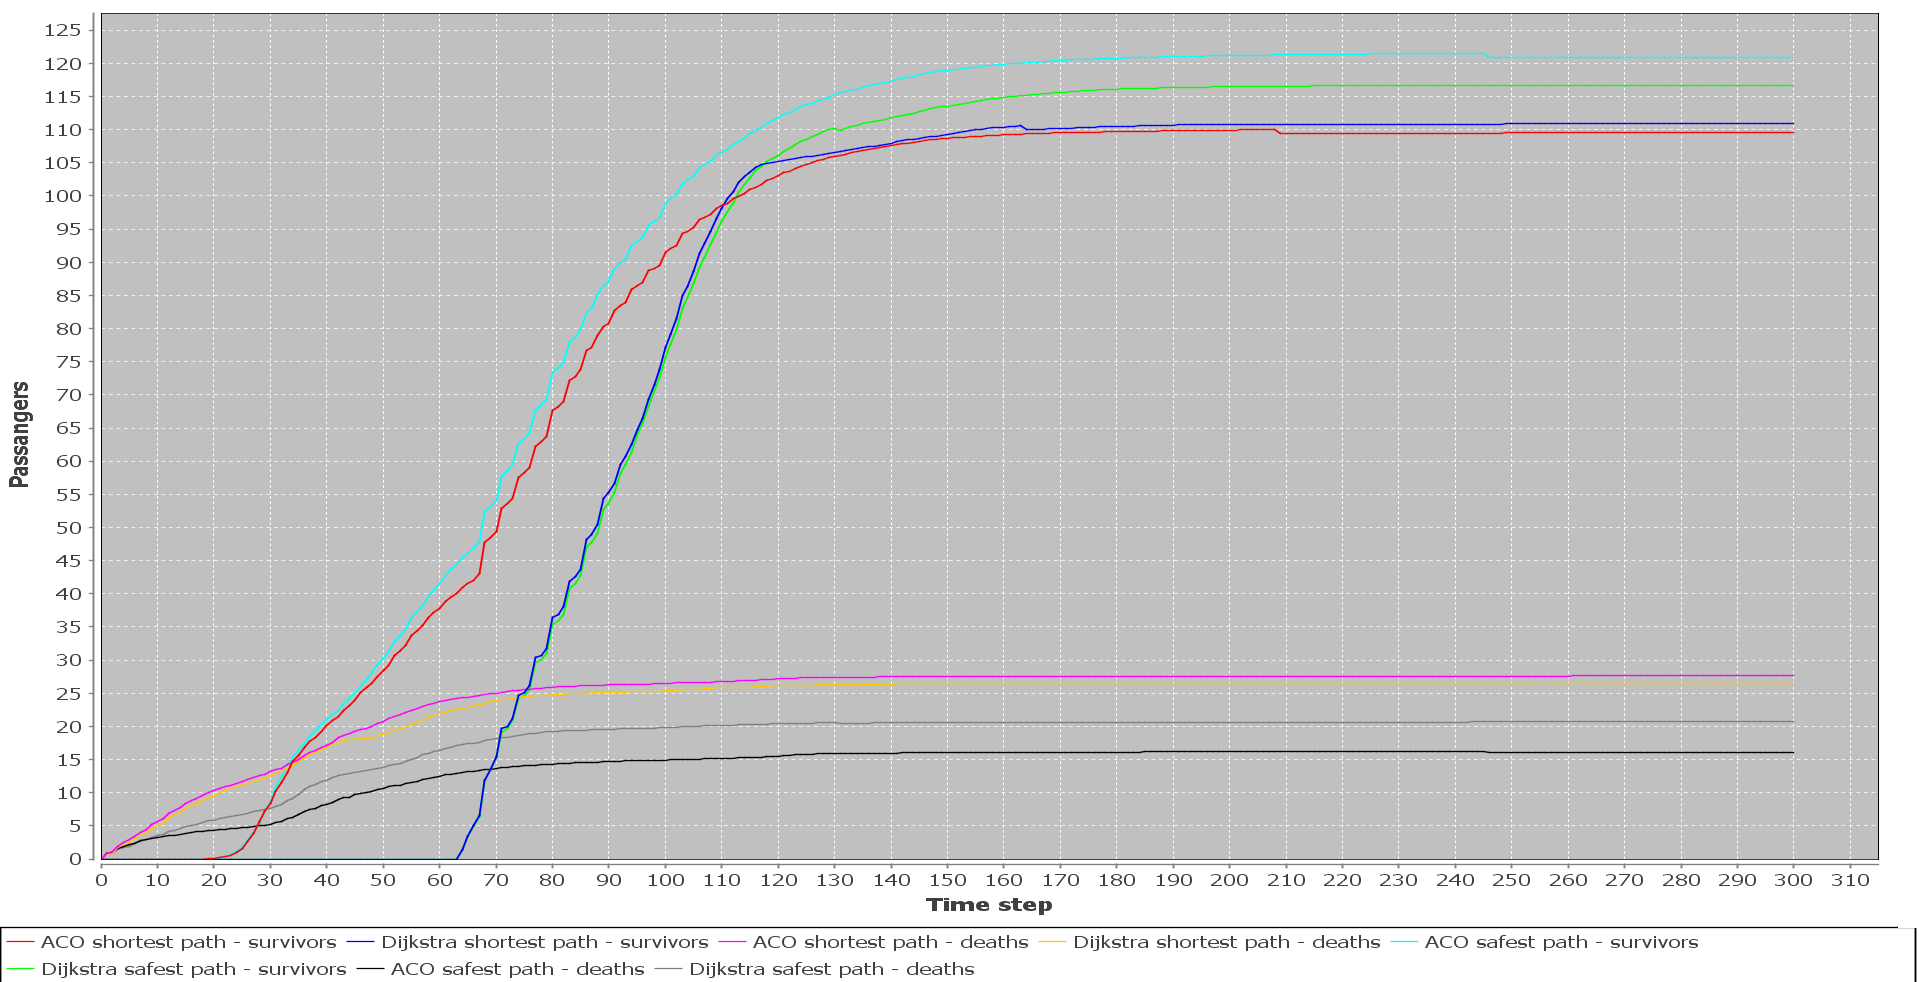
\includegraphics[scale=0.35]{images/Graph-using-1000-rounds-140-passangers-and-one-fire-dijkstra-one-time.png}
\caption{Running Dijkstra only at start.}
\label{fig:celebDF}
\end{figure}

\subsubsection{Djikstra at each time step.}
In \ref{fig:celeb} it is clearly seen that Dijkstra going for the safest path has the best results overall. ACO going for safest would be the second best algorithm followed by Dijkstra going for quickest. In the end is ACO going for quickest path, as it has problem finding the quickest path and getting the passengers off the ship before the hazards spread out to much and gets to deadly.

If you look at quickest paths only, it is clearly shown that ACO's passengers are dying more rapidly then Dijkstra's passengers. This is a good indication on that both algorithms are choosing different paths. As shortest path is measured in shortest time needed rather then shortest way to exit, it may be that Dijkstra spread the passengers more out then ACO. Also Dijkstra is getting them to an exit faster too.

If we looked at safest paths taken only, then Dijkstra is slightly increasing in saving more passengers then ACO is, or Dijkstra's passengers are dying not as fast as ACO's passengers in this case. However it is a much smaller difference here then when looking at when taking the quickest paths.



%you can see how well the different algorithms did. In both cases we only used one hazard(Fire) that spread on board the ship. As shown in the graph, Dijkstra outperforms ACO in both early and late stages of this graph. In the beginning there are more passengers dying to ACO chosen path then there is in Dijkstra's chosen path, a good sign that both are finding different paths. As shortest path is measured in shortest time needed rather then shortest way to exit, it may be that Dijkstra spread the passengers more out then ACO.

%Even when more passengers are dying at the beginning of the simulations, they both have the same boost in saved passengers at each time step. The biggest problem for ACO over Dijkstra is avoiding the hazards. Shown in the graph you can see that the death toll for ACO increases faster then Dijkstra's death toll.


%In \ref{fig:celeb}, we are using the same parameters as the first one, only difference is that we are looking after the safest path rather then the shortest path for the passengers. It is clearly shown that the death toll on the passengers is far lower then the previous one. However Dijkstra proves yet again to outperform ACO in this instance. After about 30 time steps Dijkstra starts to pull ahead of ACO in number of passengers it have guided to the lifeboats. Even in number of deaths it is shown that Dijkstra is better at avoiding them. If you look at Dijkstra in both cases, the number of deaths when looking after the safest path is 50\% less when looking for the shortest path. As mention earlier that the number of rounds above 200 did not matter may be shown in the two graphs below, both of them have the same set of parameters, only to have 1000 iteration instead of 200.

\begin{figure} [float]
\centering
\hspace*{-1.0in}
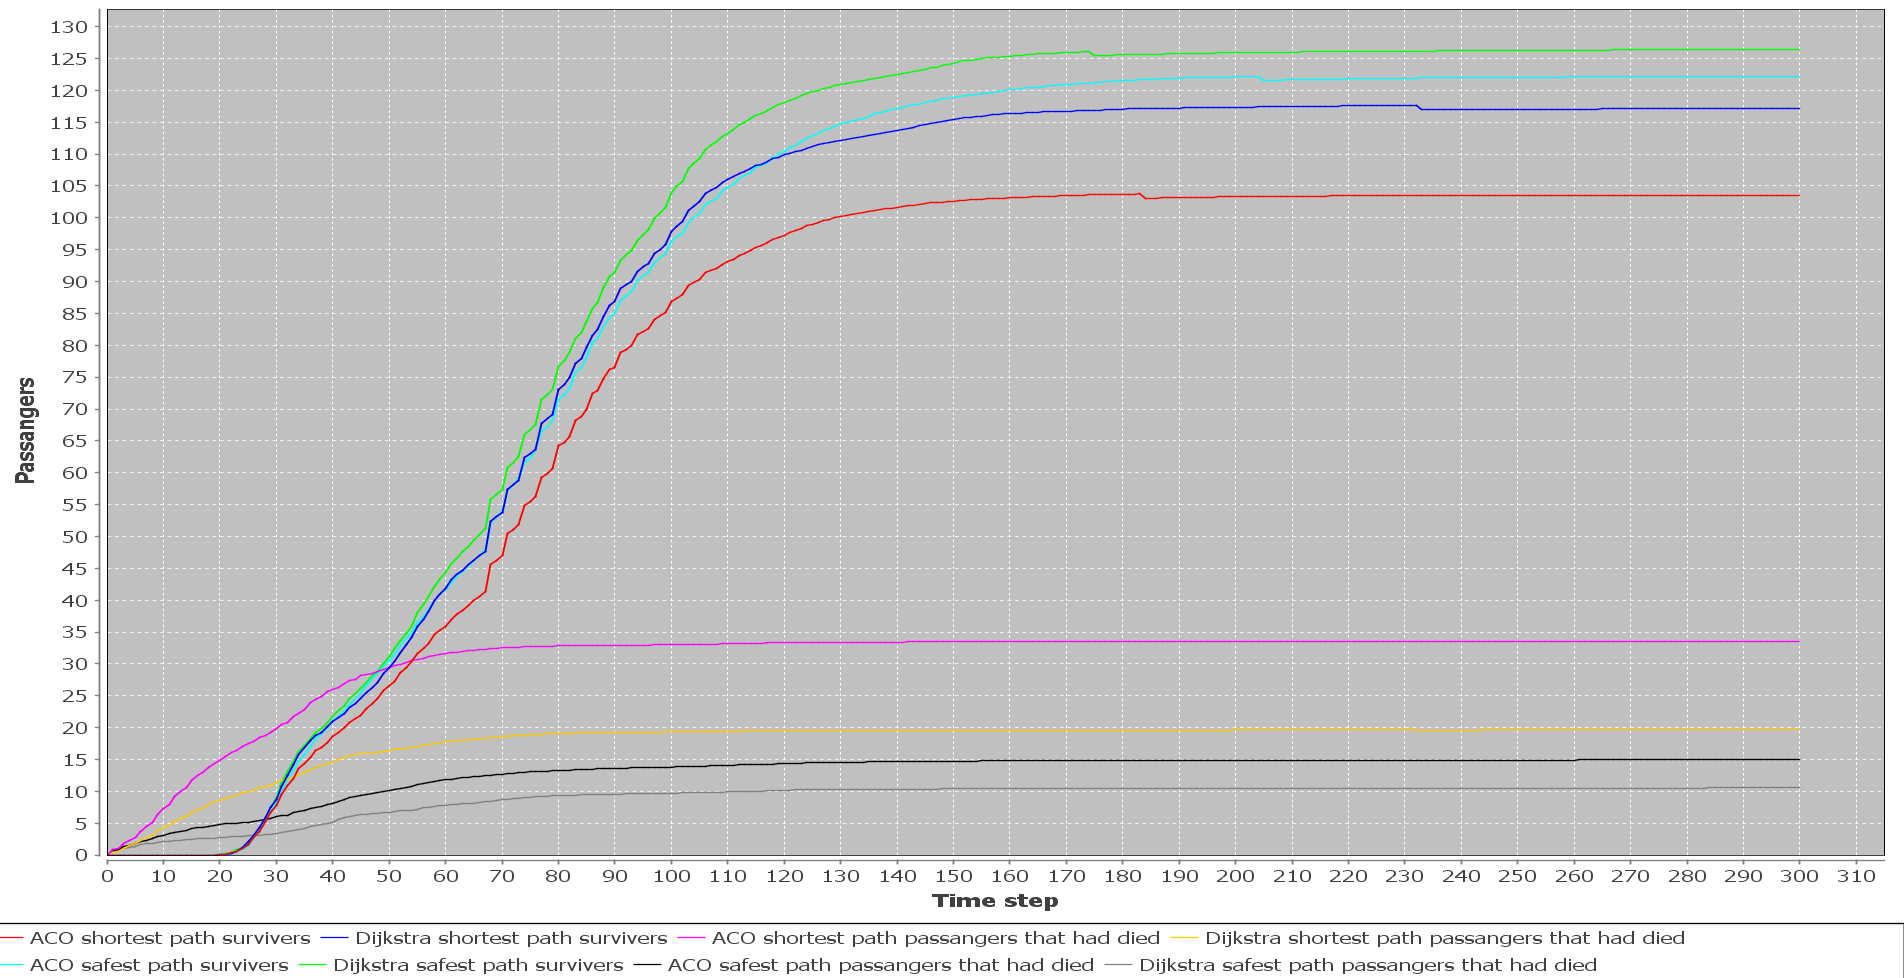
\includegraphics[scale=0.35]{images/Graph-using-200-rounds-140-passangers-and-one-fire.png}
\caption{Dijkstra and ACO running at each time step.}
\label{fig:celeb}
\end{figure}

\subsubsection{Running 1000 iterations.}
\ref{fig:celeb1000} is 1000 iterations of the simulation with same parameters as \ref{fig:celeb}, and is going for the safest route for the passengers. There is no clear difference when using 1000 iterations then 200. However Both Dijkstra and ACO when trying to find the quickest path got slightly worse then in \ref{fig:celeb}.

\begin{figure} [float]
\centering
\hspace*{-1.0in}
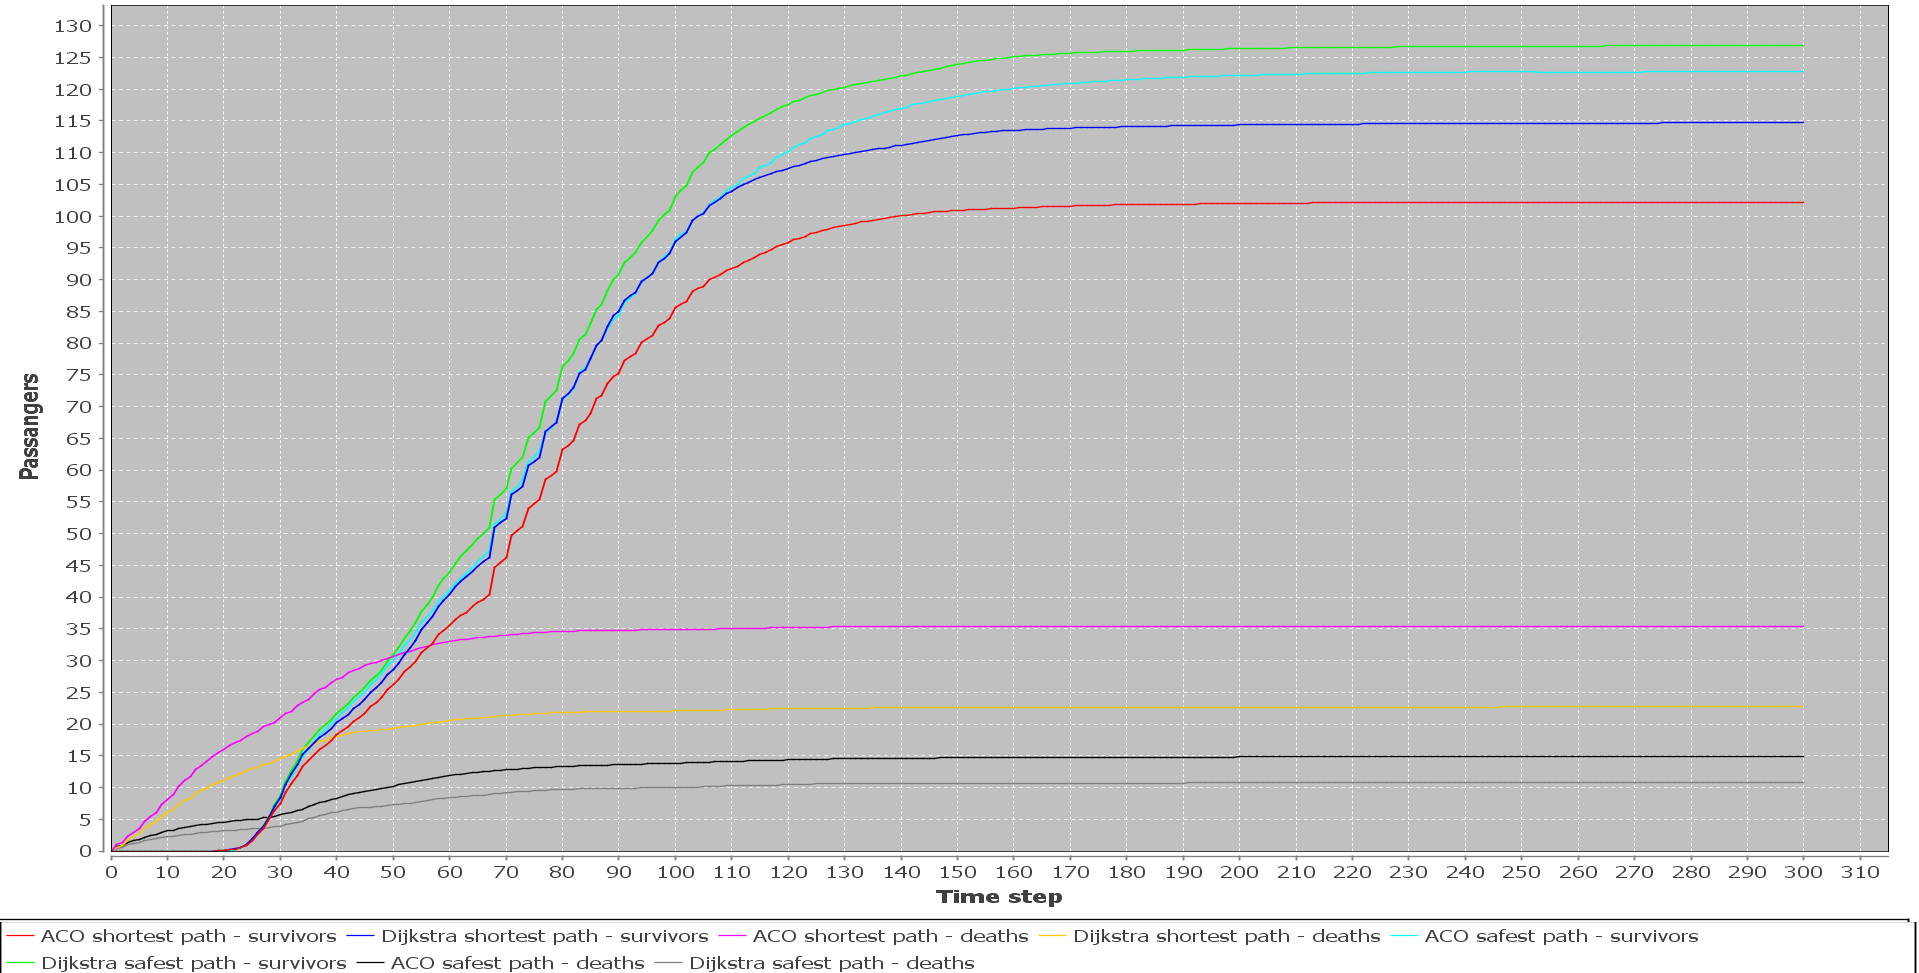
\includegraphics[scale=0.35]{images/Graph-using-1000-rounds-140-passangers.png}
\caption{Same as \ref{fig:celeb}, only using 1000 iterations.}
\label{fig:celeb1000}
\end{figure}



%In \ref{fig:celebShortPherInEdges} and \ref{fig:celebSafePherInEdges} we tested what would the difference be if we used pheromones in edges rather then in the node themselves, this showed that the ACO preformed better then our other simulations. It was compared to Dijkstra to control that there was not something special happening. The main difference is when looking for the shortest path rather then the safest. When looking for the safest there are only some small difference in both simulations.
\subsubsection{Pheromones in edges.}
In \ref{fig:celebPherInEdge} we tested what would the difference be if we used pheromones in edges rather then in the node themselves, this showed that the ACO preformed just as good when going for the safest path, however when ACO was trying to go for the quickest path this had an positive effect on it and preformed better.

\begin{figure} [float]
\centering
\hspace*{-1.0in}
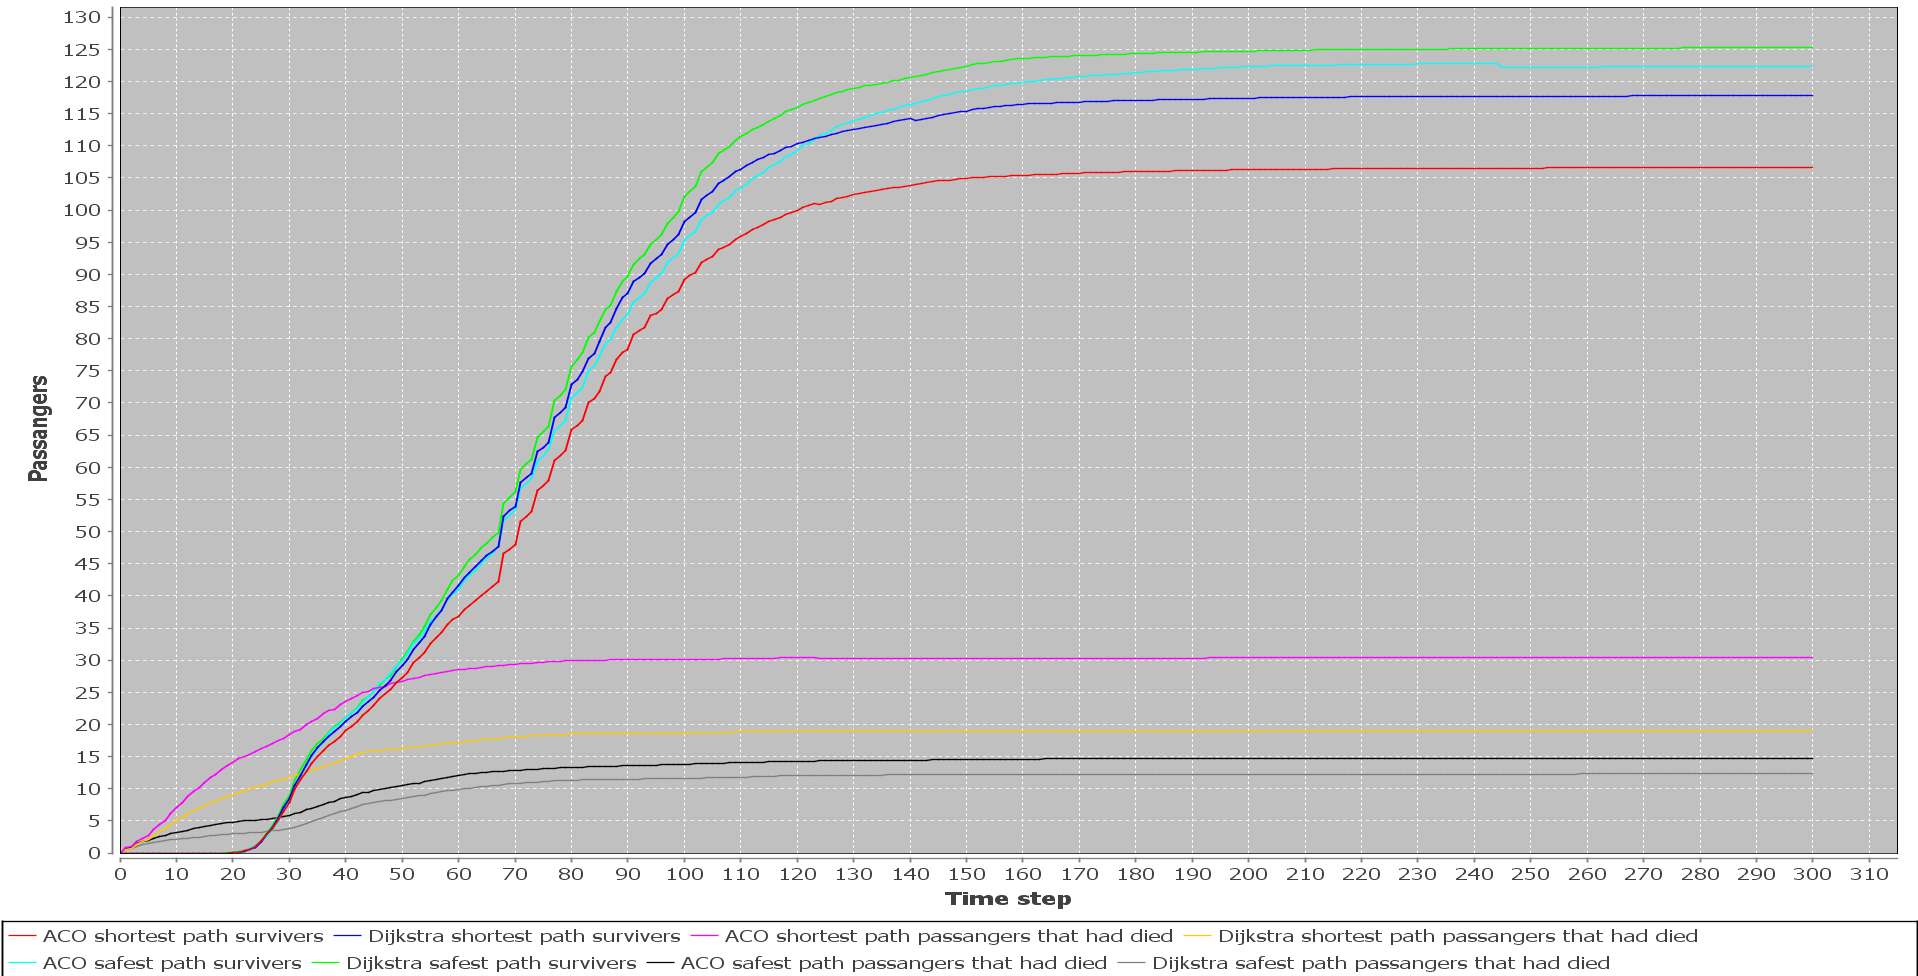
\includegraphics[scale=0.35]{images/Graph-using-200-rounds-140-passangers-and-one-hazzard-and-ACO-having-pheremons-in-edges.png}
\caption{Taking shortest path with pheromones in edges.}
\label{fig:celebPherInEdge}
\end{figure}


\subsubsection{High panic chance on passengers.}
When the chance of panic changed to a higher chance both algorithms struggled more to guide the passengers to safety. Dijkstra took the hit hardest as it sometimes it would send it one direction, then panic and go back, therefore taking a long time before that passenger got to safety or died. It is not clearly shown in this graph, however when it simulation was running, it resulted in a data file almost on a size of one 1 GB, where ACO's data file would not pass 60 MB. However it was also Dijkstra that preformed best overall, shown in \ref{fig:celebHPanic}.

\begin{figure} [float]
\centering
\hspace*{-1.0in}
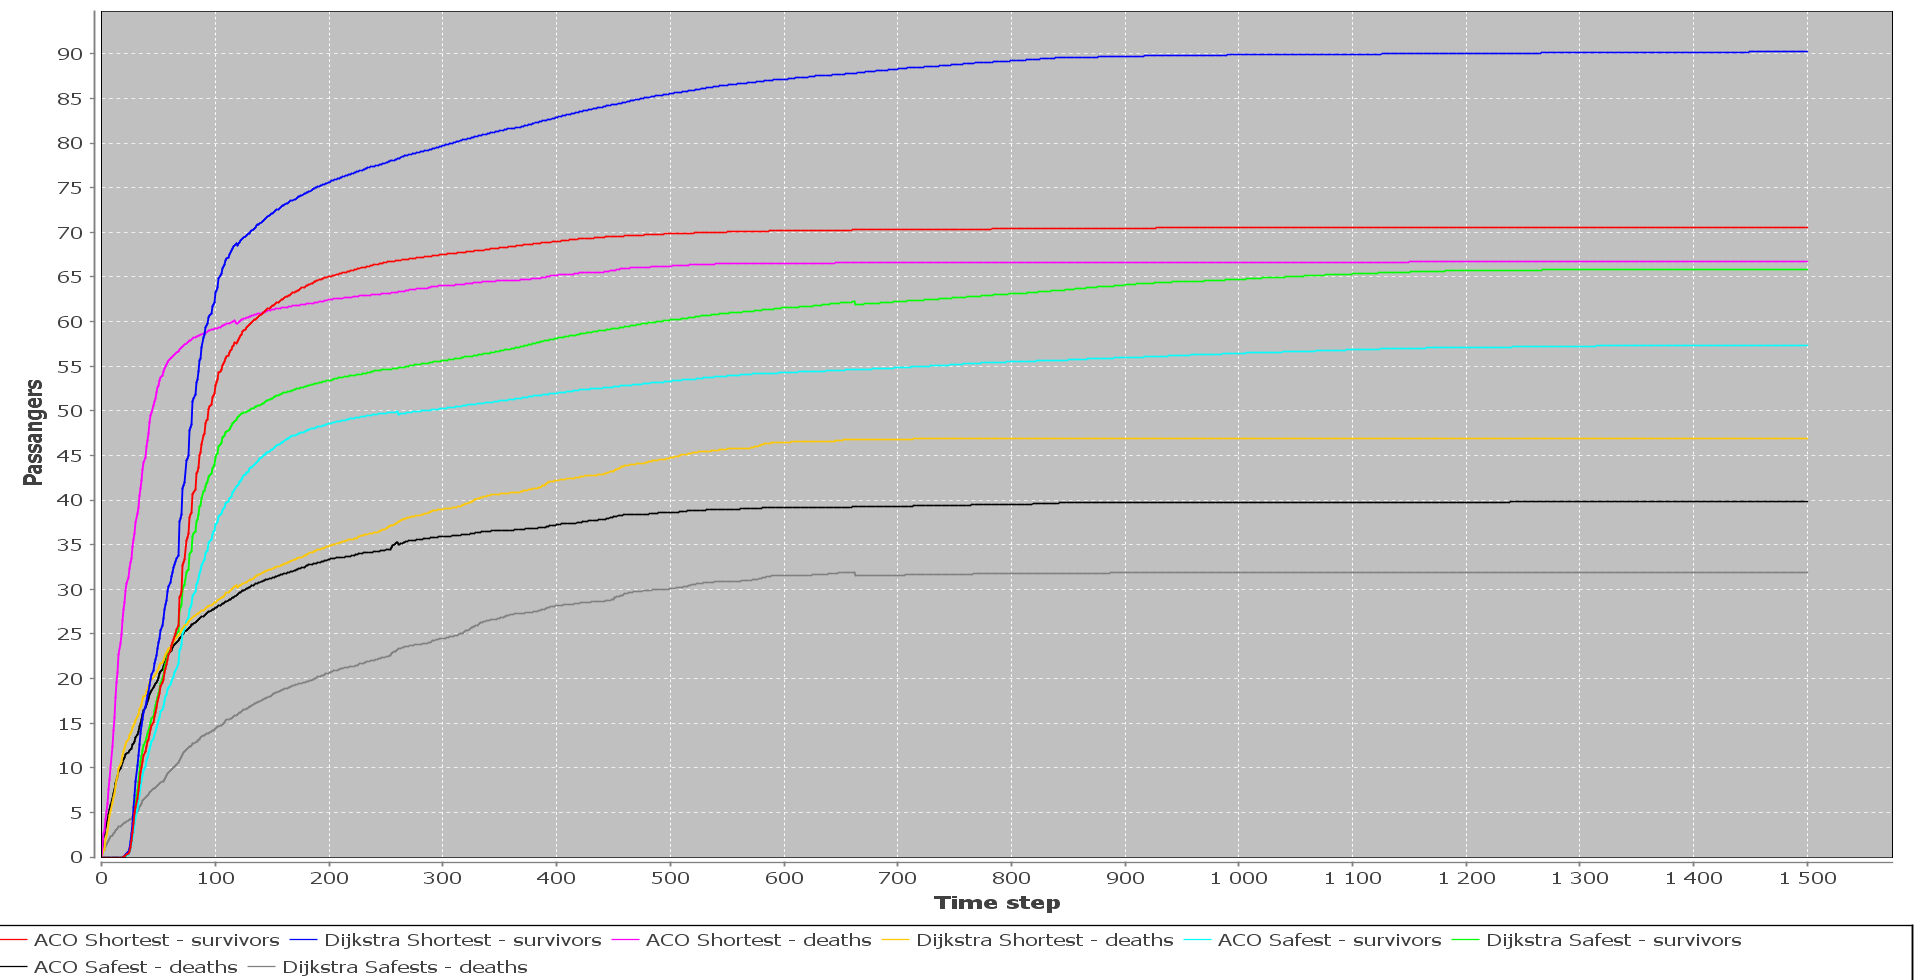
\includegraphics[scale=0.35]{images/Graph-using-200-rounds-140-passangers-and-one-fire-high-panic.png}
\caption{Taking shortest path with pheromones in edges.}
\label{fig:celebHPanic}
\end{figure}


\subsubsection{50 passengers only}

In \ref{fig:celeb50} all the different algorithms are close together and preform well when there are less passengers on board the ship. The order of witch algorithm that is best still remains the same, however Dijkstra going for quickest paths is just as good as ACO going for safest for a while, before ACO goes past it. When looking at the deaths of the passengers ACO going for safest is always much better then Dijkstra going for Quickest.

Again ACO's going for the quickest path is that it is a bit to slow and therefore the hazards have time to spread more out and create more dangerously areas.

\begin{figure} [float]
\centering
\hspace*{-1.0in}
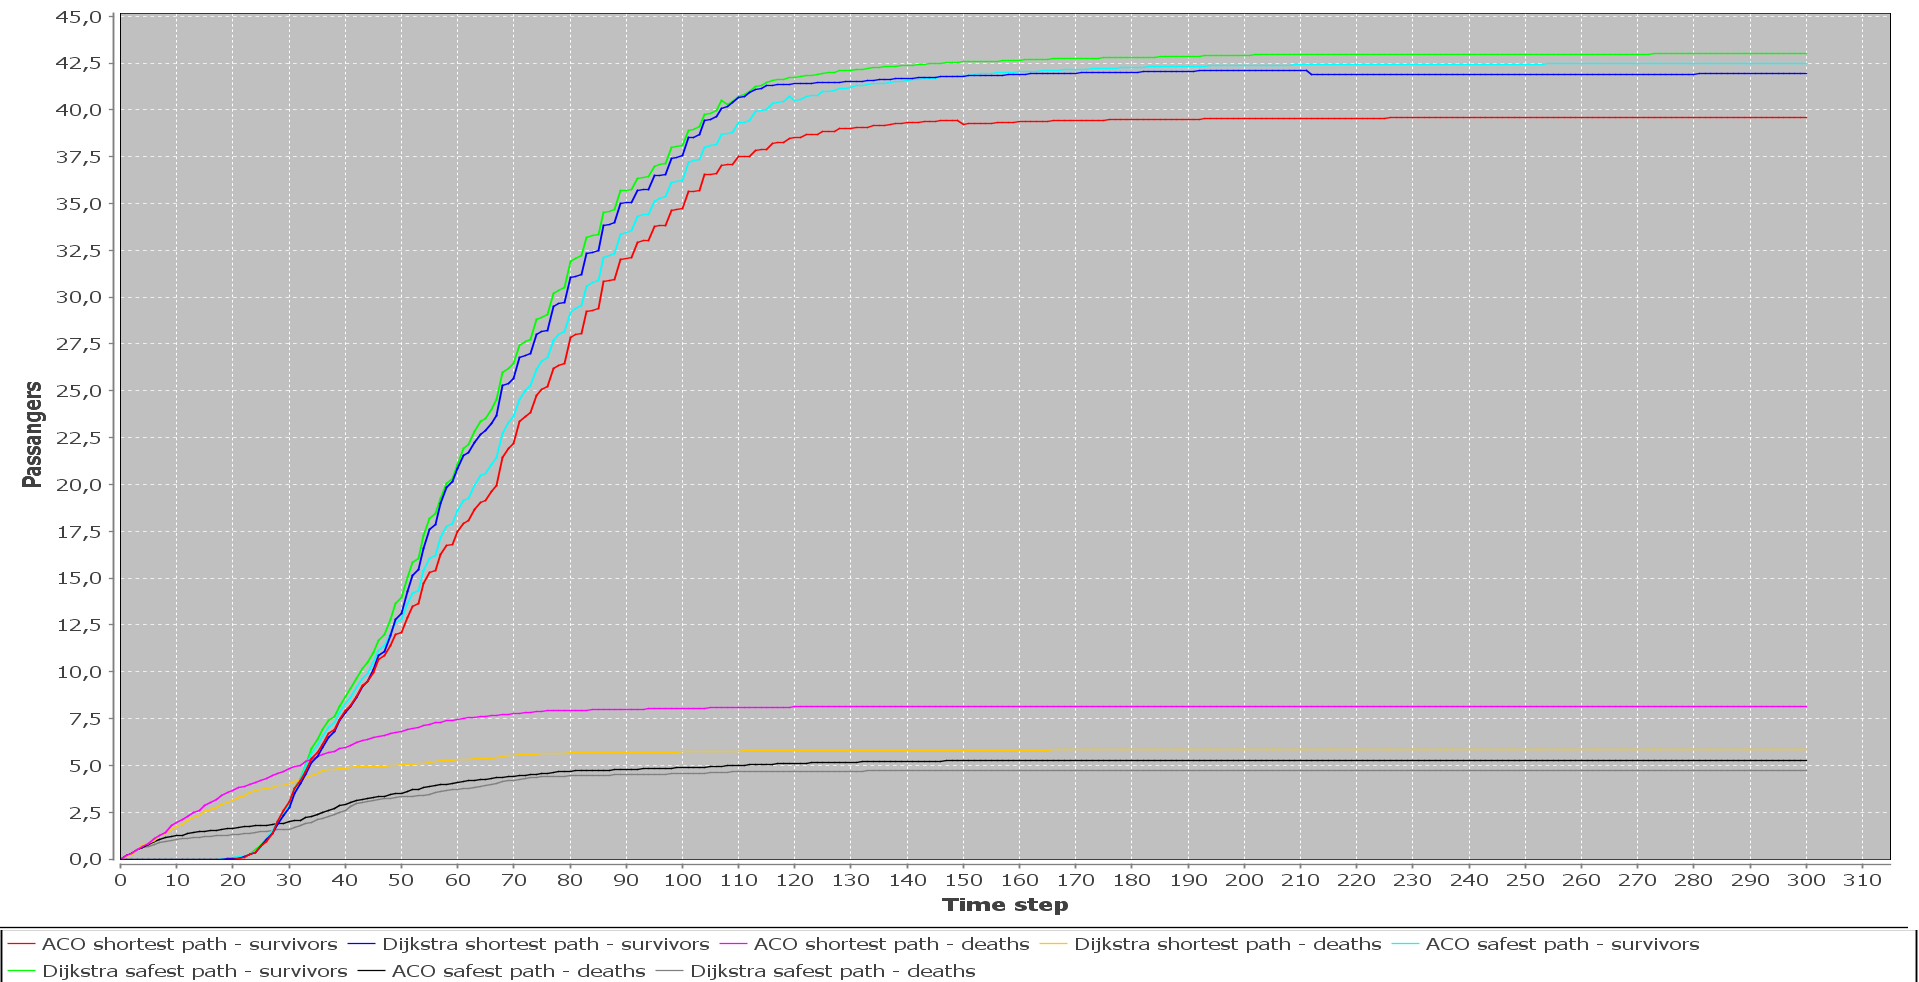
\includegraphics[scale=0.35]{images/Graph-using-200-rounds-50-passangers.png}
\caption{Taking shortest path with pheromones in edges.}
\label{fig:celeb50}
\end{figure}

\subsubsection{Slow hazards}

When comparing \ref{fig:celebSfire} to \ref{fig:celeb}, the algorithms overall did much better then all the other simulations. This was expected as the hazards moved more slowly then in all the other simulations. It is also worh noting that when finding the quickest path ACO had the biggest increase in performance, however it is still the one that is the worst off.

\begin{figure} [float]
\centering
\hspace*{-1.0in}
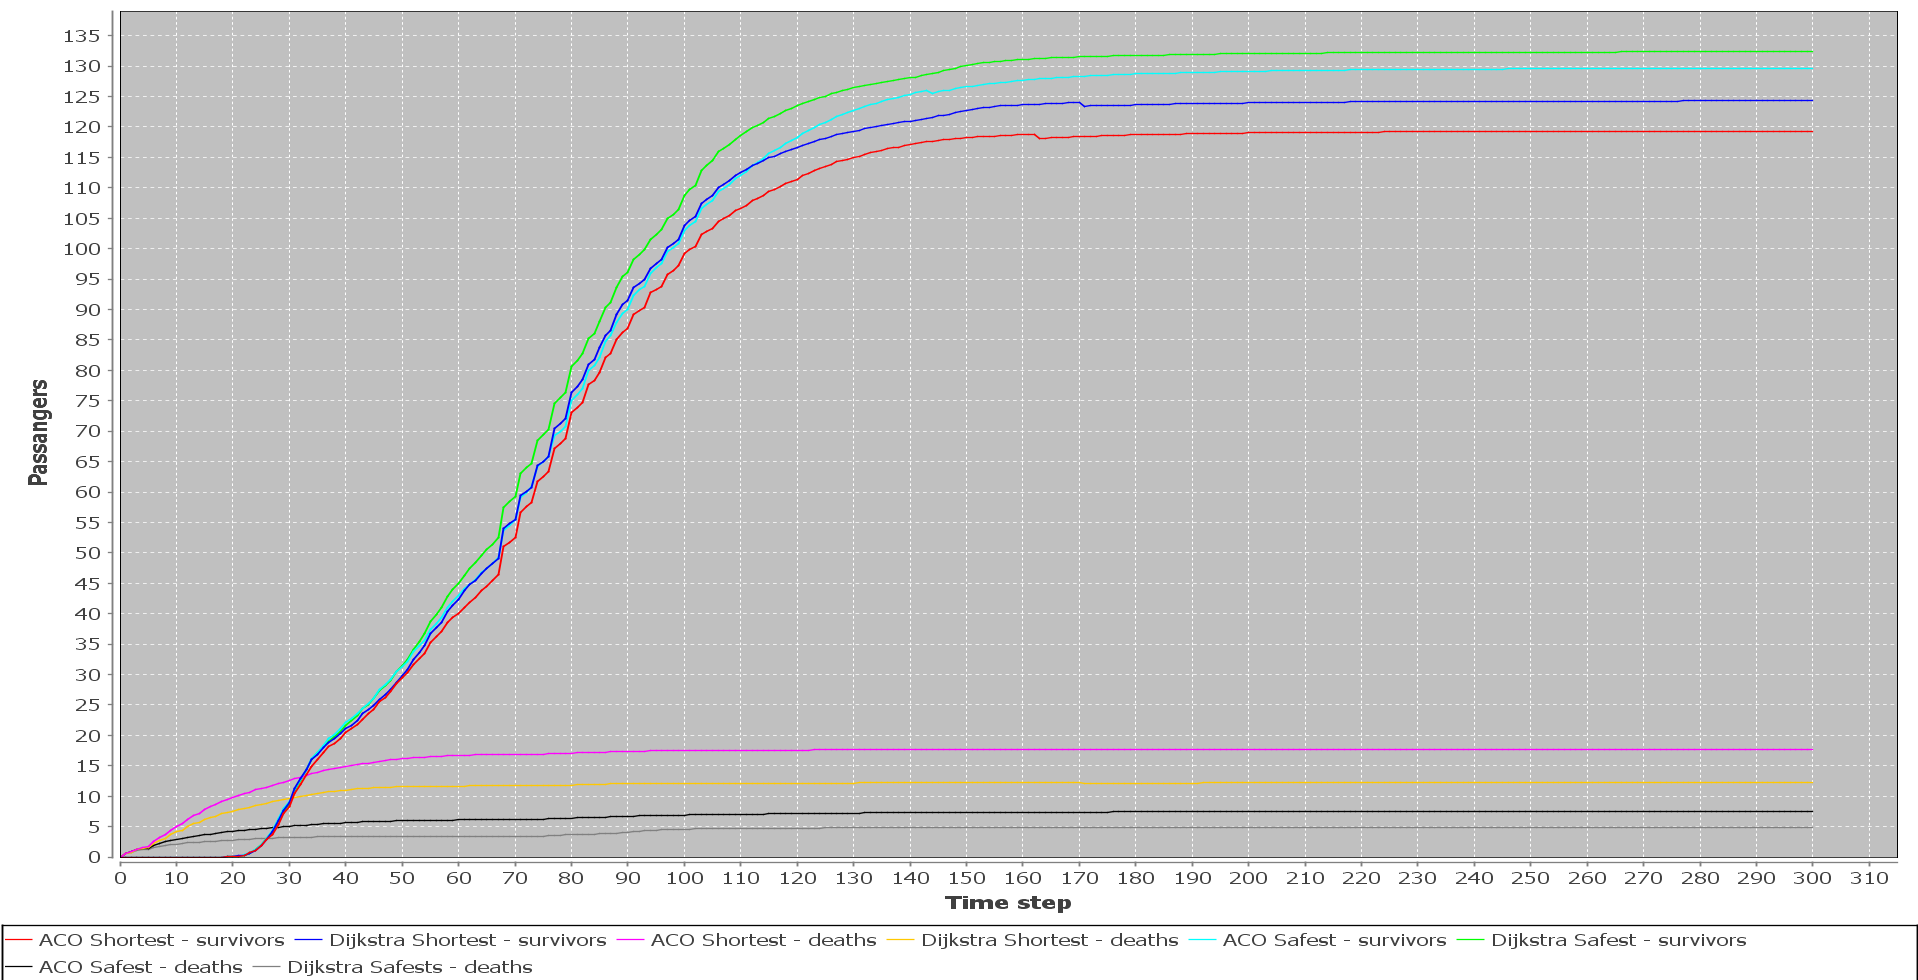
\includegraphics[scale=0.35]{images/Graph-using-200-rounds-140-passangers-slow-fire.png}
\caption{Taking shortest path with pheromones in edges.}
\label{fig:celebSfire}
\end{figure}